\subsubsection{Probabilistic Shaping}

Probabilistic shaping is a technique utilised for increasing spectral
efficiency within an optical communications system. Symbols are transmit via
probabilistic shaping by using non-uniform probabilities (outcomes have unequal
probabilities of occurring). Constellation points are distributed, using these
non-uniform probabilities, along the complex plane, in contrast to simpler square
quadrature amplitude modulation (QAM) constellation points, which are on a square
grid. When implemented alongside QAM this technique has been demonstrated
experimentally to give greatly increased sensitivity\cite{prob_2016}\cite{400Gbps_2019}.

\par Shaping allows for sensitivity gains of up to 0.8dB within optical
communications systems utilising 16QAM and 64QAM. In order to implement the
shaping within the system, the following probability mass function was applied:

\begin{equation}
	\label{eq:}
	P_x(x_i) = \frac{1}{\sum_{k=1}^{M} e^{-vx_k^2}}e^-vx_i^2 \quad
	\text{\cite{prob_2016}}
\end{equation}

\par In testing for mismatched SNR, the variation of SNR of 11dB was shown to not
require any modifications to the input distribution\cite{prob_2016}. This study
concluded that due to the robustness, sensitivity, and transmission distance
improvements gained from using shaping, that probabilistic shaping is ``highly
suitable for a practical application in optical communications systems''.

\par The benefits attributed to probabilistic shaping were also found in a study on
spectral efficiency in a 400Gb/s optical communications system, which found that
with probabilistic shaping alongside 64QAM, a 50\% ``reach'' improvement was
achieved over system in which probabilistic shaping was not
implemented\cite{400Gbps_2019}.

\par This study compares the efficiencies of a ``PS'' (Probabilistic Shaping)
system, versus that of a hybrid-QAM system. Hybrid QAM utilises multiple,
time-interleaved QAM's in order to improve the performance of regular QAM's. The
Maxwell-Boltzmann distribution shown below was used for the distribution of the
PS constellation points.

\begin{equation}
	\label{eq:}
	P_x(x_i) =
	\frac{\exp(-v(Re(x_i)^2+Im(x_i)^2))}{\sum_{k=1}^{M}\exp(-v(Re(x_k)^2+Im(x_k)^2))}  \quad
	\text{\cite{400Gbps_2019}}
\end{equation}

The experimental setup used, as shown in Figure \ref{fig:pstest}, shows the
utilisation of DSP techniques for the pre-transmission processing of the signal.
The input data is initially mapped to PS-64QAM symbols. These are then passed
through a pre-distortion (using look-up-tables) and pre-equalization stage. This
pre-equalization stage is composed of a 21-tap constant modulus algorithm (CMA)
Finite-Impulse-Response (FIR) filter\cite{400Gbps_2019}.

\begin{figure}[H]
	\centering
	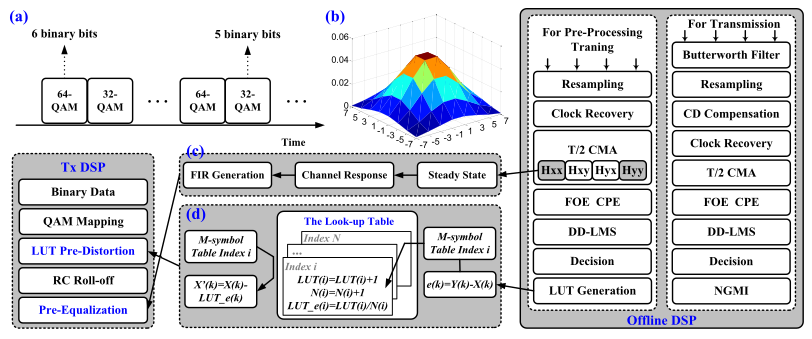
\includegraphics[width=0.8\textwidth]{images/PStest}
	\caption{Experimental Setup as in \cite{400Gbps_2019}}
	\label{fig:pstest}
\end{figure}

Due to the lower optical signal to noise ratio (OSNR) achieved using
probabilistic shaping, a transmission rate of 400Gb/s was achieved over a
transmission distance of 3,600km, a 50\% increase over the maximum transmission
distance achieved when using a hybrid-QAM system\cite{400Gbps_2019}.
